\documentclass[11pt,a4paper]{article}
\usepackage{polski}
\usepackage[utf8]{inputenc}
\usepackage{fancyhdr}
\usepackage{array}
\usepackage{algorithm}
\usepackage{graphicx}
\usepackage{algpseudocode}
\pagestyle{fancy}
\fancyhf{ }
\title{Sterownik domowy}
\author{Sebastian Brzezinka, Mietek}
\date{}
\fancyfoot[C]{\thepage}
\fancyhead[R]{Dokumentacja: Sterownik domowy}
\begin{document}
	\maketitle
	\pagebreak
	\section{Wstęp:}
	\subsection{Przeznaczenie:} 
	Sterownik przeznaczony jest do zdalego i scentralizowanego zarządzania urządzeniami elektrycznymi poprzez wlączanie ich i wyłaczanie. 
	Sterownik zaprojektowany jest z myslą o zarządzaniu światłem oraz urządzeniami RTV/AGD. 
	Drógorzędna funkcją sterownika jest odczyt danych z czujników do niego podłączonych(temperatura, wilgotność, ciśnienie ...).
	\subsection{Parametry:}
	Podstawowe parametry:\newline 
	- obsługa do 2 urządzeń za pośrednictwem portów OUT;\newline
	- obsługa do 2 czójników za pośrednictwem protów IN;\newline
	- prezentacja wyników pobranych z portów IN;\newline
	- prezentacja aktualnie włączonych urządzeń;\newline
	- ekran LCD słóżący do prezentacji wyników; \newline 
	- zarządzanie sterownikiem przy urzyciu telefonu z systemem Android;\newline
	\section{Urzytkowanie:}
	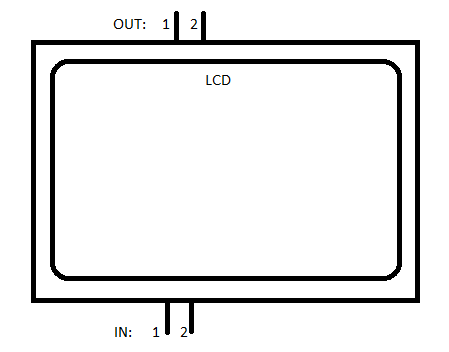
\includegraphics[]{sterownikdomowy}\newline
	\pagebreak
	Sterownik obsługiwany jest za pomocą dotykowego wyświetlacza, który pełni rolę wejścia/wyjścia. 
	Na ekranie znajdują się cztery przyciski odpowiadające kolejnym portom, zegar oraz przycisk umożliwiający parowanie urządzenia z telefonem.
	Informacje o aktywności danego portu przekazywane są poprzez zmianę koloru przycisku. \newline 
	-przycisk "OUT 1" odpowiada za przejście do panelu konfiguracyjnego portu "OUT 1";\newline
	-przycisk "OUT 2" odpowiada za przejście do panelu konfiguracyjnego portu "OUT 2";\newline
	-przycisk "IN 1" odpowiada za przejście do panelu konfiguracyjnego portu "IN 1";\newline
	-przycisk "IN 2" odpowiada za przejście do panelu konfiguracyjnego portu "IN 2";\newline
	\subsection{Panele konfiguracyjne:}
	\subsubsection{OUT:}
	Po podłączenia urządzenia do portu OUT <nr> staje się aktywyny przycisk "OUT <nr>", co pozwala na przejście do panelu administracyjnego.
	Panel administracyjny pozwala na włączenie/wyłączenie zasilania urządzenie podpiętego do danego portu.
	Panel pozwala również na ustalenie przedziału czasowego, w którym urządzenie jest włączone. 
	Dodatkową opcją panelu jest możliwość sprawdzenia poboru energii urządzenia podpiœtego do portu.
	Istnieje też możliwość ustalenia parametru uruchomienia zewnętrznego urządzenia w zależności od danych zczytanych z sensorów. 
	\subsubsection{IN:}
	Po naciśnięci przycisku "IN <nr>" wyświetlone zostają informacje o sensorze orz dane przekazane do urządzenia przez sensor.
	W panelu tym znajduje się przycisk umozliwiający odłączenie zasilania od czójnika. 
	
\end{document}
